\documentclass[12pt]{article}
\usepackage[utf8]{inputenc}
\usepackage[brazilian,provide=*]{babel}
\usepackage{sbc-template}
\usepackage{graphicx,url}
\usepackage{amsmath,amssymb}
\usepackage{booktabs}
\usepackage{multirow}
\usepackage{xcolor}
\usepackage{hyperref}
\usepackage{microtype}
\usepackage{float}
\usepackage{caption}
\usepackage{amsmath}

\sloppy
\raggedbottom

% ─────────────────────────────────────────────────────────────────────────────
\title{QML-IDS em Open RAN sob Restrições NISQ}

\author{Diego Abreu\inst{1}, Murilo Silva\inst{1}, Fiterling Sousa\inst{1},  Fernando Farias\inst{1}}

\address{Rede Nacional de Ensino e Pesquisa -- RNP
\email{\{diego.abreu,  murilo.silva, firterlinge.sousa, fernando.farias\}@rnp.br}}


\begin{document}
\maketitle

% ─── Resumo ──────────────────────────────────────────────────────────────────
\begin{resumo}
O Open RAN vem se consolidando como arquitetura para redes privadas e comerciais 5G/6G ao reduzir custos e complexidade operacional. Contudo, sua desagregação entre hardware e software amplia a superfície de ataque, sobretudo pelo uso de interfaces abertas entre funções virtualizadas. Este trabalho propõe e avalia um \textit{pipeline} de detecção de intrusão para O-RAN baseado em aprendizado de máquina clássico e quântico. Utiliza-se o conjunto público \textit{Netslab-5G-ORAN-IDD}, com 1,7 milhão de registros e seis classes de tráfego. Após pré-processamento e seleção de características, são comparados cinco classificadores clássicos e três abordagens quânticas: QKSVM, VQC e QIK-SVM. Também são avaliados modelos de ruído NISQ, aplicados heuristicamente à matriz de kernel com parâmetros inspirados em \textit{backends} IBM Quantum. Com repetições e barras de incerteza, o QKSVM atinge $93{,}9\% \pm 1{,}2\%$ de acurácia binária (desempenho pareado consistentemente acima do SVM-RBF em 10 de 10 repetições, $+0{,}85 \pm 0{,}56$~pp) e degrada entre $1{,}6$ e $3{,}3$~pp de acurácia binária sob os quatro cenários de ruído avaliados (baseline sem ruído $93{,}1\% \pm 1{,}1\%$). O canal \textit{dephasing} (T2) foi o mais prejudicial, reduzindo a acurácia binária para $87{,}8\% \pm 1{,}5\%$ em $p=0{,}05$, por afetar as coerências exploradas pelo \textit{ZZFeatureMap}. Em contraste, o VQC não convergiu em nenhuma das repetições e teve desempenho médio ($67{,}1\% \pm 4{,}4\%$) inferior ao de uma baseline majoritária.
\end{resumo}

% \begin{abstract}

% Open RAN has emerged as a standard architecture for the deployment of private and commercial 5G/6G networks, reducing the complexity and CAPEX and OPEX costs of mobile networks. However, this disaggregation between hardware and software exposes the architecture components to more network attacks due to the need for network functions to communicate via open interfaces. This work proposes and evaluates a \textit{pipeline} for intrusion detection (IDS) in the O-RAN architecture, integrating classical and quantum machine learning. For this work, we use the public dataset \textit{Netslab-5G-ORAN-IDD}, with \(1.7\)~million records and six traffic classes as the training dataset. After preprocessing and feature selection, we compare five classical classifiers and three quantum approaches: QKSVM, VQC, and QIK-SVM. We also evaluate NISQ noise models applied heuristically to the kernel matrix, with parameters inspired by IBM Quantum \textit{backends}. With repetitions and uncertainty bars, QKSVM reaches \(93.9\% \pm 1.2\%\) binary accuracy (paired advantage of \(+0.85 \pm 0.56\)~pp over SVM-RBF, 10 of 10 repetitions) and degrades by \(1.6\)--\(3.3\)~pp under the four noise scenarios evaluated. \textit{Dephasing} (\(T_2\)) was the most harmful channel, reducing accuracy to \(87.8\% \pm 1.5\%\) at \(p=0.05\). In contrast, VQC failed to converge in any repetition and underperformed a majority-class baseline on average.
% \end{abstract}

\section{Introdução}
\label{sec:intro}

%A arquitetura \textit{Open RAN} (O-RAN) representa uma transformação fundamental nas redes de %acesso via rádio, substituindo soluções proprietárias monolíticas por componentes %disagregados, interfaces abertas e controle inteligente baseado em software~\cite{oran2021}. %Embora essa abertura promova inovação e redução de custos, ela expande significativamente os %pontos de ataque: as interfaces abertas (E2, O1, A1), os componentes virtualizados (O-CU, O-%DU, O-RU) e os \textit{xApps} no \textit{near-RT RIC}, constituem novos vetores de %intrusão~\cite{openireland2024}.

A arquitetura \textit{Open RAN} (O-RAN) representa uma verdadeira mudança de paradigma para as redes de acesso via rádio. Ao deixar para trás as antigas soluções proprietárias e monolíticas, o modelo aposta na separação de componentes, no uso de interfaces abertas e em um controle inteligente guiado por software~\cite{oran2021}. No entanto, a mesma flexibilidade que impulsiona a inovação e reduz os custos também acaba ampliando a superfície de ataques da rede. Na prática, as interfaces de comunicação (E2, O1, A1), os elementos virtualizados (O-CU, O-DU, O-RU) e os \textit{xApps} rodando no \textit{near-RT RIC} criam novas portas de entrada para possíveis invasões.

%A detecção de intrusão em O-RAN impõe requisitos severos: o \textit{near-RT RIC} opera com latência inferior a 10~ms, o tráfego é heterogêneo e os padrões de ataque evoluem continuamente. O \textit{Quantum Machine Learning} (QML) emerge como alternativa promissora para problemas com estrutura de alta dimensão. Circuitos quânticos parametrizados, como o \textit{ZZFeatureMap}, mapeiam dados clássicos para espaços de Hilbert de dimensão exponencial de $2^n$, para $n$ qubits, potencialmente revelando separabilidade não acessível a kernels clássicos~\cite{havlicek2019}. Contudo, os computadores quânticos atuais operam na era NISQ, com ruído de gate, decoerência e erros de leitura que degradam os circuitos~\cite{preskill2018}.
%

A detecção de intrusão em redes O-RAN apresenta desafios rigorosos: além de o tráfego ser altamente heterogêneo e os padrões de ataque evoluírem continuamente, o \textit{near-RT RIC} exige tempos de resposta entre 10~ms a 1~s. Diante dessa complexidade e alta dimensionalidade dos dados, o \textit{Quantum Machine Learning} (QML) surge como uma alternativa promissora. Ao utilizar circuitos quânticos parametrizados, como o \textit{ZZFeatureMap}, torna-se possível mapear dados clássicos para espaços de Hilbert com dimensão exponencial de $2^n$ (sendo $n$ o número de \textit{qubits}). Na prática, isso pode revelar padrões de separabilidade inacessíveis aos \textit{kernels} clássicos~\cite{havlicek2019}. Apesar desse potencial, os computadores quânticos atuais operam na era NISQ (\textit{Noisy Intermediate-Scale Quantum}), sofrendo com limitações físicas como ruído nas portas lógicas, decoerência e erros de leitura. Mais criticamente, a sobrecarga temporal necessária para codificar dados clássicos e executar os circuitos quânticos reais ainda costuma exceder a rígida janela de latência de 10~ms, exigindo otimizações arquiteturais para viabilizar essa integração.

%As principais contribuições deste trabalho são: (i)~um \textit{pipeline} completo de IDS para O-RAN usando o dataset \textit{Netslab-5G-ORAN-IDD}~\cite{nidd2022}; (ii)~implementação de três algoritmos QML com simulação \textit{statevector} exata; (iii)~modelagem realista de ruído NISQ com quatro canais físicos calibrados a partir de dados reais de backends IBM Quantum; e (iv)~análise comparativa sistemática entre abordagens clássicas e quânticas com discussão de viabilidade para \textit{near-RT RIC}.

As principais contribuições deste trabalho são: (i) o desenvolvimento de um \textit{pipeline} completo de IDS para O-RAN utilizando o \textit{dataset} Netslab-5G-ORAN-IDD~\cite{nidd2022}; (ii) a implementação de três algoritmos de QML com simulação exata de vetores de estado (\textit{statevector}); (iii) um estudo de sensibilidade a ruído da era NISQ, aplicando heuristicamente quatro canais físicos à matriz de kernel com parâmetros inspirados em \textit{backends} reais da IBM Quantum (\autoref{subsec:noise_models}); e (iv) uma análise comparativa sistemática entre modelos clássicos e quânticos, com repetições e barras de incerteza, acompanhada de uma discussão crítica sobre a viabilidade prática dessas soluções operarem no \textit{near-RT RIC}.


Além desta seção introdutória, o artigo é dividido em mais seis seções. Na \autoref{sec:relacionados} -- Trabalhos Relacionados -- o texto destaca pesquisas sobre datasets O-RAN e o uso de QML, diferenciando a abordagem do estudo atual. A \autoref{sec:metodologia} -- Dataset e Metodologia -- descreve o conjunto de dados utilizado (Netslab-5G-ORAN-IDD), o processo de pré-processamento e os modelos quânticos e de ruído avaliados. Na \autoref{sec:resultados_classico} -- Resultados --  modelos clássicos, os autores apresentam o desempenho de classificadores como Random Forest e Decision Tree. Em \autoref{sec:qml} -- Resultados -- o aprendizado de máquina quântico é feita uma comparação de desempenho entre os modelos quânticos e clássicos. A \autoref{sec:ruido} -- Impacto do Ruído Quântico -- avalia a degradação dos modelos sob diferentes condições de ruído de equipamentos reais da IBM e discute a viabilidade para cenários de baixa latência (near-RT RIC). Por fim, a \autoref{sec:conclusao} -- Conclusão -- resume os achados, destacando a eficácia da abordagem quântica em amostragens reduzidas, e propõe direcionamentos para trabalhos futuros.


% ─────────────────────────────────────────────────────────────────────────────
\section{Trabalhos Relacionados}
\label{sec:relacionados}

\cite{openireland2024} apresentaram um dos primeiros datasets de KPIs O-RAN com tráfego malicioso real, incluindo cenários de DDoS e DoS sob diferentes padrões de mobilidade. \cite{nidd2022} introduziram o 5G-NIDD com fluxos gerados em infraestrutura 5G real. No campo do QML, \cite{liu2021} demonstraram que kernels quânticos podem oferecer vantagem em dados com estrutura específica, enquanto \cite{cerezo2021} discutiram desafios como \textit{barren plateaus} em VQCs (\textit{Variational Quantum Classifiers}). 

Este trabalho se distingue por aplicar QML diretamente a dados de segurança de O-RAN, avaliar a sensibilidade a múltiplos canais de ruído heurísticos com parâmetros inspirados em hardware real e fornecer uma comparação direta e repetida (com incerteza) entre QKSVM (\textit{Quantum Kernel Support Vector Machine}), VQC e métodos clássicos.


% ─────────────────────────────────────────────────────────────────────────────
\section{Dataset e Metodologia}
\label{sec:metodologia}

Para estruturar a avaliação do pipeline de detecção de intrusões na arquitetura O-RAN, esta seção detalha os procedimentos metodológicos e as ferramentas adotadas no estudo. Inicialmente, descrevemos as características do conjunto de dados Netslab-5G-ORAN-IDD e as etapas rigorosas de pré-processamento necessárias para adequar os dados de tráfego de rede às restrições dimensionais dos algoritmos. Em seguida, apresentamos a formulação das abordagens de classificação quântica e de inspiração quântica avaliadas na pesquisa, como o QKSVM e o VQC. Por fim, detalhamos os canais de ruído aplicados heuristicamente sobre a matriz de kernel para estudar a sensibilidade dos modelos a imperfeições típicas da era NISQ, com parâmetros inspirados em dispositivos reais da IBM Quantum


\subsection{Conjunto de Dados}

O \textit{Netslab-5G-ORAN-IDD} contém 1.723.817 registros com 26 atributos de fluxos TCP/UDP/ICMP. A Tabela~\ref{tab:dataset} sumariza a distribuição das classes.

\begin{table}[H]
\centering
\caption{Distribuição das classes no dataset Netslab-5G-ORAN-IDD.}
\label{tab:dataset}
\small
\begin{tabular}{lrrl}
\toprule
\textbf{Categoria} & \textbf{Registros} & \textbf{\%} & \textbf{Tipos de ataque} \\
\midrule
DoS        & 632.507 & 36,7\% & SYN flood, HTTP flood \\
DDoS       & 420.282 & 24,4\% & UDP, TCP ACK, ICMP, Slowloris \\
Web        & 288.304 & 16,7\% & XSS, SQL injection, dir. bruteforce \\
Probe      & 183.293 & 10,6\% & TCP/UDP portscan, OS fingerprinting \\
Benigno    & 170.865 &  9,9\% & HTTP, SSH, DNS, NTP \\
Bruteforce &  28.566 &  1,7\% & SSH, FTP \\
\bottomrule
\end{tabular}
\end{table}

A Tabela \ref{tab:dataset} evidencia que o conjunto Netslab-5G-ORAN-IDD contempla uma ampla variedade de cenários de ataque, abrangendo desde negação de serviço, varredura e comprometimento de aplicações Web até tentativas de força bruta contra serviços autenticados. As classes DoS e DDoS concentram o maior volume de registros, refletindo ataques voltados à indisponibilidade de recursos de rede, enquanto as categorias Web, Probe e Bruteforce representam, respectivamente, vetores de exploração de aplicações, reconhecimento da infraestrutura e tentativa de acesso indevido por repetição de credenciais. Já a classe Benigno reúne tráfego legítimo de serviços amplamente utilizados, servindo como referência para a distinção entre comportamento normal e malicioso. Em conjunto, essas categorias tornam o dataset particularmente adequado para avaliar a capacidade de modelos clássicos e quânticos em identificar padrões heterogêneos de intrusão em redes O-RAN.



%Removemos identificadores de fluxo (\texttt{uid}, \texttt{src\_ip}, \texttt{dst\_ip}), aplicamos transformação $\log(1+x)$ às colunas de bytes e criamos quatro características derivadas: \texttt{byte\_ratio}, \texttt{pkt\_ratio}, \texttt{bytes\_per\_pkt\_src} e \texttt{bytes\_per\_pkt\_dst}. Um Random Forest auxiliar selecionou as 15 características mais relevantes. Para os modelos clássicos utilizamos 120.000 amostras (20.000/classe); para QML, 1.500 amostras (250/classe), necessário dado o custo $\mathcal{O}(N^2 \cdot 2^n)$ do kernel quântico.

No pré-processamento, removemos seis atributos de identificação direta dos fluxos e de rótulos redundantes: \texttt{uid}, \texttt{src\_ip}, \texttt{dst\_ip} e \texttt{history} (identificadores/quase-identificadores do ambiente de coleta), além de \texttt{attack\_type} e \texttt{traffic\_type} (rótulos de granularidade diferente da variável-alvo \texttt{attack\_category} -- \texttt{traffic\_type} é, na prática, a própria tarefa binária, e \texttt{attack\_type} é uma versão mais granular de \texttt{attack\_category}; ambos foram excluídos do conjunto de preditores para evitar vazamento de rótulo). Em seguida, aplicamos a transformação
$\log(1+x)$ às variáveis relacionadas a bytes, reduzindo a assimetria das distribuições e suavizando a influência de valores extremos. Também criamos quatro características derivadas — \texttt{byte\_ratio}, \texttt{pkt\_ratio}, \texttt{bytes\_per\_pkt\_src} e \texttt{bytes\_per\_pkt\_dst} — com o objetivo de sintetizar relações relevantes entre volume e estrutura do tráfego, o que tende a enriquecer a representação dos fluxos para fins de classificação.

Após essa etapa, um \textit{Random Forest} auxiliar (\texttt{n\_estimators=100}, \texttt{max\_depth=10}, semente 42) foi utilizado para ranquear a relevância das variáveis e selecionar as 15 características mais informativas: \texttt{dst\_port}, \texttt{http\_status\_error}, \texttt{conn\_state\_enc}, \texttt{log\_dst\_bytes}, \texttt{src\_port}, \texttt{duration}, \texttt{log\_files\_total\_bytes}, \texttt{dst\_bytes}, \texttt{bytes\_per\_pkt\_dst}, \texttt{log\_src\_ip\_bytes}, \texttt{src\_ip\_bytes}, \texttt{is\_file\_transfered}, \texttt{files\_total\_bytes}, \texttt{byte\_ratio} e \texttt{log\_dst\_ip\_bytes}. Colunas categóricas (\texttt{proto}, \texttt{service}, \texttt{conn\_state}) foram convertidas por \textit{label encoding} antes dessa etapa. Para os modelos clássicos, trabalhamos com 120.000 amostras, distribuídas igualmente entre as classes (\autoref{sec:resultados_classico}), enquanto para os experimentos de QML utilizamos 1.500 amostras (250 por classe), uma decisão necessária diante do custo \(O(N^2 \cdot 2^n)\) do kernel quântico, que cresce rapidamente com o número de amostras e com a quantidade de qubits.

Dentre as 15 características selecionadas, os experimentos quânticos (\autoref{sec:qml} e \autoref{sec:ruido}) usam apenas $n=6$, uma por \textit{qubit} do \textit{ZZFeatureMap}. Essa segunda redução também foi feita por importância do \textit{Random Forest} (\texttt{n\_estimators=200}, \texttt{max\_depth=10}, semente 42), agora treinado apenas sobre as 15 características candidatas e a variável-alvo multiclasse, das quais retivemos as seis mais importantes: \texttt{dst\_port} (0,137), \texttt{conn\_state\_enc} (0,116), \texttt{http\_status\_error} (0,099), \texttt{src\_port} (0,085), \texttt{duration} (0,063) e \texttt{log\_dst\_bytes} (0,062) -- valores entre parênteses são a importância normalizada do RF. Todas as seis foram reescaladas para $[0,\pi]$ com \texttt{MinMaxScaler} antes da codificação quântica, faixa compatível com os ângulos de rotação $R_z$ da \autoref{eq:zzfeaturemap}.

\textbf{Limitação da divisão treino/teste:} tanto os experimentos clássicos quanto os quânticos particionam os dados com \texttt{train\_test\_split} aleatório estratificado por classe, sem controle por sessão/captura de origem, e o dataset não disponibiliza um identificador de captura que permitisse uma divisão por grupo. Verificamos que, considerando as 15 características selecionadas, $17.714$ dos $120.000$ registros ($14{,}8\%$) são duplicatas exatas de outro registro da amostra -- uma fração substancial que a divisão aleatória por registro não impede de ser compartilhada entre treino e teste. Assim, as métricas relatadas neste trabalho estimam a capacidade de interpolação nos cenários de captura já observados, e não a generalização para novas capturas de rede; essa limitação é mais severa do que uma divisão aleatória "genérica" sugeriria, dado o volume de duplicatas identificado.



\subsection{Modelos Quânticos}

\textbf{ZZFeatureMap e QKSVM:} O QKSVM utiliza um kernel quântico para medir similaridade entre amostras após sua codificação em estados quânticos. Neste trabalho, empregamos uma codificação com $n=6$ qubits e $R=2$ repetições. A operação de codificação é definida por:


\begin{equation}
U_\phi(x) =
\prod_{r=1}^{R}
\left[
\prod_{q=1}^{n}
\left(H_q \cdot R_z^{(q)}(2x_q)\right)
\cdot
\prod_{(q,k) \in S}
\mathrm{CNOT}_{q,k}\
\cdot
R_z^{(k)}\left(2(\pi - x_q)(\pi - x_k)\right)
\cdot
\mathrm{CNOT}_{q,k}
\right]
\label{eq:zzfeaturemap}
\end{equation}


A primeira parte do circuito aplica portas de Hadamard e rotações $R_z$ dependentes dos atributos de entrada. Em seguida, as portas CNOT e rotações condicionadas introduzem correlações entre pares de qubits. Assim, o \textit{ZZFeatureMap} não codifica apenas atributos individuais, mas também interações não lineares entre eles. Essa propriedade é relevante para IDS, pois muitos ataques são caracterizados por combinações de métricas, e não por um único atributo isolado. O kernel quântico mede a fidelidade entre os estados codificados:
\begin{equation}
K(x_a, x_b) =
\left|\langle \phi(x_a) | \phi(x_b) \rangle\right|^2, \quad
\mathbf{K} = \left|\Phi^\dagger \Phi\right|^2,
\label{eq:kernel}
\end{equation}
onde $\Phi \in \mathbb{C}^{N \times 2^n}$ contém os estados quânticos das $N$ amostras. A matriz $\mathbf{K}$ é então usada por um SVM clássico, substituindo kernels tradicionais como RBF.

\textbf{VQC:} O \textit{Variational Quantum Classifier} combina uma etapa de codificação com um circuito variacional treinável. Utilizamos o \textit{ZZFeatureMap} com uma repetição, seguido de $L=2$ camadas de rotações $R_y$ e $R_z$ e portas CNOT em anel. A saída do modelo é dada por $p(1|x) = (1-\langle Z_0\rangle)/2$, e os parâmetros são otimizados via COBYLA. Diferentemente do QKSVM, que depende de uma matriz de kernel, o VQC tenta aprender diretamente os parâmetros do circuito. Isso reduz a dependência de uma matriz quadrática em $N$, mas introduz desafios de otimização, especialmente em circuitos ruidosos ou com gradientes pequenos.

\textbf{QIK-SVM:} O QIK-SVM é uma abordagem \textit{quantum-inspired}, isto é, inspirada em mecanismos de codificação quântica, mas executada inteiramente em hardware clássico. Utilizamos uma codificação inspirada em Fourier, $\varphi(u) = [\cos u, \sin u, \cos 2u, \sin 2u]$, seguida de um kernel RBF no espaço transformado. Essa abordagem tem custo de inferência $\mathcal{O}(1)$ por transformação de atributo, tornando-se atraente para cenários com restrição de latência, ainda que não reproduza completamente a geometria induzida pelo \textit{ZZFeatureMap}.

\subsection{Modelos de Ruído NISQ}
\label{subsec:noise_models}

Aplicamos à matriz de kernel ideal transformações heurísticas inspiradas em canais NISQ para estudar a sensibilidade do classificador; os resultados desta seção não equivalem à execução dos circuitos nos \textit{backends} IBM. Concretamente, avaliamos quatro canais aplicados diretamente sobre os valores de $K(i,j)$, e não sobre o \textit{statevector} ou o circuito transpilado. Não há, portanto, transpilação para o conjunto de portas nativas de cada dispositivo, modelagem de conectividade (\textit{coupling map}) nem erro de leitura (\textit{readout}) por qubit -- apenas os quatro canais a seguir, aplicados de forma fechada sobre o kernel. O expoente $d$ usado nas fórmulas abaixo representa o número médio de portas de dois qubits do \textit{ZZFeatureMap} ($d=20$ para $n=6$ qubits e $R=2$ repetições, contado diretamente na Eq.~\ref{eq:zzfeaturemap}: $n{-}1=5$ pares de CNOTs por repetição, 2 CNOTs por par, 2 repetições), não um parâmetro calibrado por dispositivo.

\textbf{Depolarizante:} $K_\mathrm{dep}(i,j) = \alpha^d \cdot K(i,j) + (1-\alpha^d)/2^n$, com $\alpha = 1-4p/3$. Esse canal representa uma perda geral de informação quântica, aproximando o estado de uma distribuição mais uniforme. Na matriz de kernel, isso reduz o contraste entre pares de amostras semelhantes e diferentes, tornando a separação entre classes menos evidente.

\textbf{Dephasing (T2):} $K_\mathrm{deph}(i,j) = e^{-p\cdot d} \cdot K(i,j)$, $i \neq j$ — destrói as coerências de fase entre qubits. Esse canal é particularmente relevante para o \textit{ZZFeatureMap}, pois parte da separabilidade entre as classes é codificada em relações de fase. Assim, quando o \textit{dephasing} aumenta, o kernel perde informação discriminativa importante, o que pode degradar diretamente o desempenho do QKSVM.

\textbf{Amortecimento de amplitude (T1):} $K_\mathrm{amp}(i,j) = f^d \cdot K(i,j) + (1-f^d)/2^n$, com $f = 1-\gamma/2$. Esse ruído modela a tendência de relaxação dos qubits para o estado fundamental. Em comparação ao \textit{dephasing}, seu impacto tende a ser mais brando neste estudo, pois ele não ataca diretamente as coerências de fase exploradas pelo mapa de características, embora ainda possa reduzir a expressividade da representação quântica.

\textbf{Shot noise:} $K_\mathrm{shot}(i,j) \sim \mathcal{N}\left(K(i,j), K(i,j)(1-K(i,j))/N_\mathrm{shots}\right)$. Esse ruído representa a variabilidade estatística causada por um número finito de medições. Em hardware quântico real, as probabilidades não são observadas diretamente, mas estimadas a partir de múltiplas execuções do circuito. Portanto, quanto menor o número de \textit{shots}, maior a incerteza na estimativa dos elementos da matriz de kernel. Após perturbar cada entrada, a matriz é explicitamente simetrizada ($K_n \leftarrow (K_n + K_n^\top)/2$) e a diagonal é fixada em 1. Essa simetrização não garante, porém, que $K_n$ permaneça semidefinida positiva: ao perturbar cada entrada de forma independente, o ruído gaussiano pode produzir autovalores negativos, de modo que $K_n$ deixa de ser, em geral, um kernel de Mercer válido. O SVM com \texttt{kernel="precomputed"} do scikit-learn não verifica essa propriedade antes do ajuste; tratamos essa limitação como uma aproximação aceitável para o estudo de sensibilidade proposto, mas ela deve ser corrigida (por exemplo, por projeção no cone semidefinido positivo) em trabalhos futuros que pretendam interpretar $K_n$ como um kernel fisicamente válido.

Os parâmetros dos modelos de ruído foram calibrados com dados públicos de três \textit{backends} IBM Quantum: ibm\_brisbane 2024, ibm\_kyoto 2023 e ibm\_nairobi 2022. Também incluímos um cenário \textit{Noisy extreme}, com níveis de ruído mais elevados, para avaliar o comportamento do QKSVM em condições adversas. Os quatro canais são aplicados em sequência (depolarizante $\rightarrow$ \textit{dephasing} $\rightarrow$ amortecimento de amplitude $\rightarrow$ \textit{shot noise}) sobre a mesma matriz $K$, e não de forma independente.


% ─────────────────────────────────────────────────────────────────────────────
\section{Resultados: Modelos Clássicos}
\label{sec:resultados_classico}

A Tabela~\ref{tab:classico} apresenta os resultados dos classificadores clássicos. O \textit{Random Forest} obteve o melhor desempenho geral (F1-macro = 94,99\%), seguido do \textit{Gradient Boosting}. A \textit{Decision Tree} atingiu 94,65\% de F1-macro com o menor tempo de ajuste do lote de treino entre os cinco modelos (coluna "Tempo treino+pred."). As classes \textit{probe} e \textit{web} atingem precisão e revocação próximas a 100\%, enquanto \textit{benign} e \textit{bruteforce} apresentam maior confusão mútua — tráfego de bruteforce (SSH/FTP) compartilha padrões de bytes com tráfego legítimo.

\begin{table}[H]
\centering
\caption{Desempenho dos classificadores clássicos (120.000 amostras, split 80/20). A coluna de tempo mede o ajuste (\texttt{fit}) sobre as 96.000 amostras de treino somado à predição em lote sobre as 24.000 de teste -- \emph{não} é uma medida de latência de inferência por fluxo.}
\label{tab:classico}
\small
\begin{tabular}{lcccccc}
\toprule
\textbf{Modelo} & \textbf{Acc.} & \textbf{F1-macro} & \textbf{F1-w} & \textbf{Acc. (bin.)} & \textbf{F1 (bin.)} & \textbf{Tempo treino+pred.} \\
\midrule
Decision Tree       & 94,58\% & 94,65\% & 94,65\% & 96,67\% & 98,02\% & 0,4s \\
Random Forest       & \textbf{94,92\%} & \textbf{94,99\%} & \textbf{94,99\%} & \textbf{96,97\%} & \textbf{98,21\%} & 5,7s \\
Gradient Boosting   & 94,67\% & 94,73\% & 94,73\% & 96,54\% & 97,95\% & 116s \\
Logistic Regression & 80,68\% & 80,69\% & 80,69\% & 93,85\% & 96,43\% & 2,1s \\
KNN ($k=5$)         & 93,58\% & 93,66\% & 93,66\% & 96,20\% & 97,74\% & 1,2s \\
\bottomrule
\end{tabular}
\end{table}

Ressaltamos que a coluna de tempo da Tabela~\ref{tab:classico} não deve ser lida como latência de inferência por fluxo: ela mede o tempo de \texttt{fit} sobre todo o lote de treino somado ao \texttt{predict} em lote sobre o teste, medido em uma única execução, sem separar treino de predição nem medir o tempo por amostra individual. Nenhuma medição de latência ponta a ponta (por fluxo, sob concorrência, ou com comunicação de rede) foi realizada neste trabalho; comparações com a janela de 10~ms do \textit{near-RT RIC} feitas nas seções seguintes devem ser lidas como indicativas de ordem de grandeza, não como validação de viabilidade operacional.


% ─────────────────────────────────────────────────────────────────────────────
\section{Resultados: Aprendizado de Máquina Quântico}
\label{sec:qml}

\subsection{Comparativo QML vs.\ clássico}

O simulador \textit{statevector} foi implementado em NumPy com $n=6$ qubits ($2^6=64$ dimensões). Os experimentos utilizam 1.500 amostras (250 por classe, split 75/25). Diferentemente da versão original deste trabalho, que reportava uma única execução, repetimos cada experimento $R=10$ vezes com reamostragem completa dos dados a cada repetição (semente $42, 43, \ldots, 51$) -- exceto o VQC, repetido $R=5$ vezes dado seu custo computacional (COBYLA, 100 iterações, $\approx\!4$--$6$~min por execução). A Tabela~\ref{tab:qml} reporta média $\pm$ desvio-padrão. Incluímos também uma baseline majoritária (que sempre prediz a classe mais frequente) e o F1-macro, pois a tarefa binária é desbalanceada: $83{,}3\% \pm 0{,}1\%$ das amostras de teste pertencem à classe "ataque" (apenas \textit{benigno} é a classe negativa entre as seis categorias), o que infla a acurácia bruta de qualquer classificador razoável.

\begin{table}[H]
\centering
\caption{Comparativo QML vs.\ clássico (1.500 amostras, split 75/25, média $\pm$ desvio-padrão de $R=10$ repetições; VQC com $R=5$). Tarefa "Bin." = binária (benigno vs.\ ataque); "Multi." = multiclasse (6 classes).}
\label{tab:qml}
\small
\begin{tabular}{llccc}
\toprule
\textbf{Categoria} & \textbf{Modelo} & \textbf{Tarefa} & \textbf{Acc.} & \textbf{F1-macro} \\
\midrule
\multirow{3}{*}{Quântico}
  & QKSVM     & Bin.   & $93{,}9 \pm 1{,}2\%$ & $87{,}1 \pm 3{,}1\%$ \\
  & VQC       & Bin.   & $67{,}1 \pm 4{,}4\%$ & $57{,}4 \pm 7{,}1\%$ \\
  & QIK-SVM   & Multi. & $84{,}5 \pm 1{,}5\%$ & $84{,}4 \pm 1{,}6\%$ \\
\midrule
\multirow{3}{*}{Clássico}
  & SVM-RBF   & Bin.   & $93{,}0 \pm 1{,}0\%$ & $84{,}9 \pm 2{,}7\%$ \\
  & RF        & Multi. & $89{,}2 \pm 1{,}0\%$ & $89{,}2 \pm 1{,}0\%$ \\
  & LR        & Bin.   & $92{,}4 \pm 1{,}3\%$ & $84{,}5 \pm 3{,}0\%$ \\
\midrule
\multirow{2}{*}{Baseline}
  & Majoritária & Bin.   & $83{,}3 \pm 0{,}1\%$ & $45{,}4 \pm 0{,}0\%$ \\
  & Majoritária & Multi. & $16{,}5 \pm 0{,}0\%$ & $4{,}7 \pm 0{,}0\%$ \\
\bottomrule
\end{tabular}
\end{table}

Em acurácia bruta, QKSVM e SVM-RBF parecem próximos ($93{,}9\%$ vs.\ $93{,}0\%$, dentro de um desvio-padrão um do outro), o que isoladamente não sustentaria uma vantagem robusta. Entretanto, como os dois modelos foram treinados e testados sobre exatamente os mesmos 10 pares treino/teste (comparação pareada), pudemos comparar diretamente por repetição: o QKSVM superou o SVM-RBF em \textbf{10 das 10 repetições}, com vantagem pareada de $+0{,}85 \pm 0{,}56$~pp de acurácia -- uma diferença pequena, mas consistente. Em macro-F1, a vantagem do QKSVM sobre o SVM-RBF é maior ($87{,}1\%$ vs.\ $84{,}9\%$), e ambos superam com folga a baseline majoritária ($45{,}4\%$ de F1-macro), confirmando que os classificadores aprendem sinal genuíno além do desbalanceamento de classes.

O \textbf{VQC} teve desempenho muito inferior ao relatado na versão original deste trabalho: em vez de uma única execução com $81{,}3\%$ de acurácia, as $R=5$ repetições produzem média de apenas $67{,}1\% \pm 4{,}4\%$ -- \emph{pior que a baseline majoritária binária} ($83{,}3\%$) -- e o otimizador COBYLA \textbf{não convergiu em nenhuma das 5 repetições} (0/5), com alta variância entre execuções (desvio-padrão de $4{,}4$~pp em acurácia e $7{,}1$~pp em F1-macro). Isso é consistente com a literatura sobre \textit{barren plateaus}~\cite{cerezo2021}, mas contradiz a leitura otimista do resultado original: o único ponto observado anteriormente (81,3\%) estava acima da média das repetições e não é representativo do comportamento típico do VQC neste problema. Concluímos que o VQC, na configuração testada ($L=2$ camadas, 100 amostras de treino, 100 iterações COBYLA), não é competitivo e sua instabilidade de otimização é uma limitação central, não um detalhe secundário.

O QIK-SVM, com custo de inferência mínimo, atinge $84{,}5\% \pm 1{,}5\%$ de acurácia multiclasse, superando a baseline majoritária multiclasse ($16{,}5\%$) por larga margem e ficando próximo do RF clássico multiclasse ($89{,}2\%$), o que sustenta seu uso como alternativa \textit{quantum-inspired} de baixo custo (\autoref{sec:ruido}).

O achado de \textbf{vantagem de amostragem} da versão original -- QKSVM $90$--$92\%$ vs.\ SVM-RBF $\approx\!83\%$ com apenas 30--50 amostras de treino -- também não se sustenta com repetição. A \autoref{fig:qml_perf} mostra a curva de aprendizado com $R=10$ repetições: em $N=30$, o QKSVM atinge $93{,}2\% \pm 0{,}7\%$ contra $89{,}7\% \pm 4{,}3\%$ do SVM-RBF -- uma vantagem média de $3{,}5$~pp, porém o desvio-padrão do SVM-RBF ($4{,}3$~pp) é seis vezes maior que o do QKSVM ($0{,}7$~pp), de modo que a diferença não é estatisticamente robusta com apenas 10 repetições (os intervalos se sobrepõem). Em $N=80$ a diferença já é inferior a $0{,}3$~pp, e em $N=120$ o SVM-RBF chega a superar ligeiramente o QKSVM. A leitura correta é: o QKSVM tende a ser mais \emph{estável} (menor variância) que o SVM-RBF quando há poucos dados de treino, mas a alegação de uma vantagem determinística de acurácia em regime de poucas amostras não é sustentada pelos dados repetidos.

\begin{figure}[H]
\centering
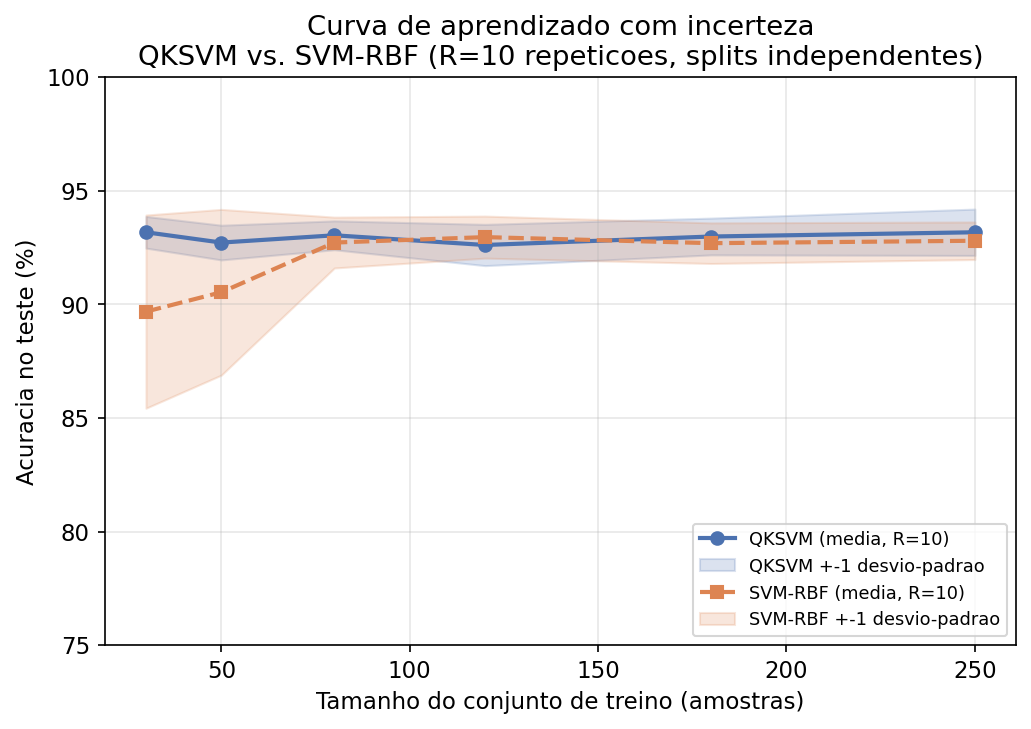
\includegraphics[width=\textwidth]{figures/fig_qml_perf.png}
\caption{Curva de aprendizado com incerteza (média $\pm$ desvio-padrão, $R=10$ repetições com reamostragem completa): QKSVM vs.\ SVM-RBF em função do tamanho do conjunto de treino.}
\label{fig:qml_perf}
\end{figure}


% ─────────────────────────────────────────────────────────────────────────────
\section{Impacto do Ruído Quântico}
\label{sec:ruido}

\subsection{Degradação por backend IBM}

Diferentemente da versão original, que usava como referência um backend "ideal" que já incluía \textit{shot noise} (com $N_\mathrm{shots}=100.000$), aqui adotamos uma \textbf{única baseline}, sem ruído algum, como referência para todos os $\Delta$ desta seção, do Resumo e da Conclusão: $93{,}08\% \pm 1{,}10\%$ (binária) e $82{,}33\% \pm 4{,}48\%$ (multiclasse), média $\pm$ desvio-padrão de $R=8$ repetições com reamostragem completa (100 amostras/classe $\times$ 6 classes = 600 amostras, split 75/25, sementes independentes). A Tabela~\ref{tab:backends_results} resume a degradação do QKSVM por backend em relação a essa baseline única.

\begin{table}[H]
\centering
\caption{Degradação do QKSVM por backend IBM em relação à baseline sem ruído (média $\pm$ desvio-padrão, $R=8$ repetições com reamostragem completa por repetição).}
\label{tab:backends_results}
\small
\begin{tabular}{lcccc}
\toprule
\textbf{Backend} & \textbf{Acc. bin.} & \textbf{$\Delta$Acc.} & \textbf{Acc. multi.} & \textbf{$\Delta$Acc. multi.} \\
\midrule
Sem ruído (baseline) & $93,08 \pm 1,10\%$ & ---         & $82,33 \pm 4,48\%$ & --- \\
ibm\_brisbane (2024) & $91,50 \pm 1,96\%$ & $-1,58$~pp  & $80,25 \pm 3,89\%$ & $-2,08$~pp \\
ibm\_kyoto (2023)    & $90,92 \pm 2,31\%$ & $-2,17$~pp  & $78,75 \pm 3,22\%$ & $-3,58$~pp \\
ibm\_nairobi (2022)  & $90,50 \pm 1,72\%$ & $-2,58$~pp  & $78,33 \pm 3,48\%$ & $-4,00$~pp \\
Noisy extreme        & $89,83 \pm 1,14\%$ & $-3,25$~pp  & $76,00 \pm 3,56\%$ & $-6,33$~pp \\
\bottomrule
\end{tabular}
\end{table}

Com essa baseline consistente, a degradação é maior do que a versão original relatava: mesmo os backends mais recentes (ibm\_brisbane, ibm\_kyoto) apresentam entre $1{,}6$ e $2{,}2$~pp de queda em acurácia binária -- e não "inferior a $1{,}6\%$" como constava anteriormente -- e entre $2{,}1$ e $3{,}6$~pp na tarefa multiclasse. O cenário \textit{Noisy extreme} chega a $-3{,}25$~pp (binária) e $-6{,}33$~pp (multiclasse). Os desvios-padrão (obtidos por reamostragem completa, não apenas por variação do \textit{shot noise}) são da mesma ordem de grandeza que os próprios $\Delta$, de modo que nenhuma dessas degradações deve ser lida como precisamente estimada; a comparação entre backends deve ser tomada de forma qualitativa (ordenamento aproximado ibm\_brisbane $<$ ibm\_kyoto $\lesssim$ ibm\_nairobi $<$ Noisy extreme), não pelo valor pontual de cada $\Delta$.

\subsection{Canal mais crítico: dephasing}

O \textit{dephasing} (T2) é o canal mais prejudicial. A \autoref{fig:noise_sweep} mostra a varredura completa de $p \in [0, 0{,}05]$ com $R=8$ repetições: em $p=0{,}05$, a acurácia binária cai para $87{,}75\% \pm 1{,}53\%$, uma queda de $-5{,}33$~pp em relação à baseline sem ruído ($93{,}08\% \pm 1{,}10\%$) -- valores próximos, mas não idênticos, à alegação "de 94,0\% para 88,0\%" da versão original, que vinha de uma única execução sem repetição nem barra de incerteza. O \textit{ZZFeatureMap} codifica a separabilidade das classes em coerências de fase entre qubits — os termos $R_z(2(\pi-x_i)(\pi-x_j))$ da Eq.~(\ref{eq:zzfeaturemap}) — e o \textit{dephasing} destrói exatamente essas coerências, o que explica por que ele é o canal mais prejudicial dentre os quatro avaliados (\autoref{subsec:noise_models}) mesmo em magnitude de ruído comparável.

\begin{figure}[H]
\centering
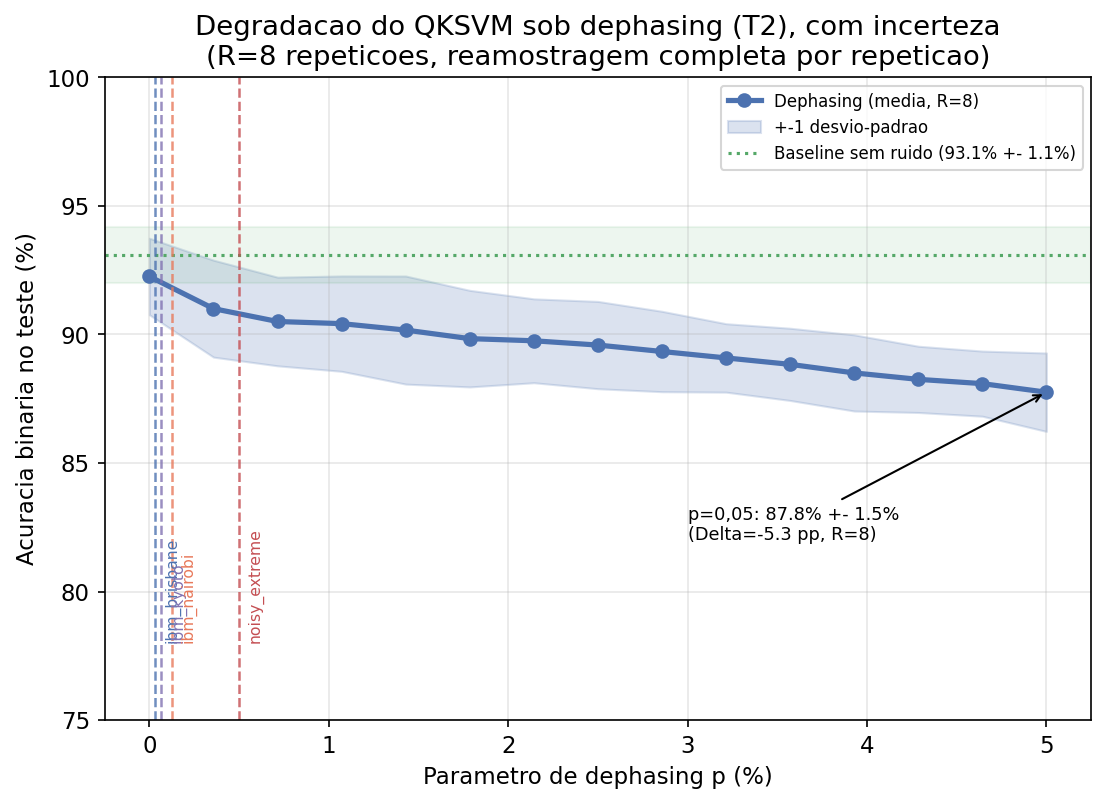
\includegraphics[width=\textwidth]{figures/fig_noise_sweep.png}
\caption{Degradação da acurácia binária do QKSVM sob o canal \textit{dephasing} em função de $p$, com banda de $\pm 1$ desvio-padrão ($R=8$ repetições). Linhas verticais marcam o parâmetro $p$ efetivo de cada \textit{backend} IBM calibrado.}
\label{fig:noise_sweep}
\end{figure}

\subsection{Viabilidade para near-RT RIC}

Não medimos latência ponta a ponta nem integração como \textit{xApp}; portanto, os resultados deste trabalho não estabelecem a viabilidade do QKSVM no \textit{near-RT RIC}. A Tabela~\ref{tab:classico} mede apenas tempo de treino somado a predição em lote (\autoref{sec:resultados_classico}), sem circuitos quânticos, contagem de \textit{shots}, comunicação entre O-CU/O-DU/near-RT RIC ou filas de processamento -- todos elementos que dominam a latência real de um \textit{xApp} de IDS. Com hardware quântico real, o custo de simulação $\mathcal{O}(2^n)$ do QKSVM deixaria de existir, mas o tempo de preparação de estado, execução do circuito e leitura em um dispositivo NISQ real não foi estimado aqui. Adicionalmente, o \textit{Netslab-5G-ORAN-IDD} contém apenas fluxos de camada de transporte (TCP/UDP/ICMP) agregados por conexão, e não KPIs nativos das interfaces O-RAN (E2, O1, A1); a aplicabilidade dos modelos a esses sinais específicos do \textit{near-RT RIC} não foi avaliada. Dentre os modelos comparados, a Decision Tree clássica é a que exige menor custo computacional de treino/predição em lote, com desempenho apenas 0,3~pp de F1-macro inferior ao RF (Tabela~\ref{tab:classico}).


% ─────────────────────────────────────────────────────────────────────────────
\section{Conclusão}
\label{sec:conclusao}

Este trabalho apresentou um pipeline de IDS para O-RAN integrando aprendizado de máquina clássico e quântico, com avaliação de sensibilidade a ruído NISQ aplicada heuristicamente sobre a matriz de kernel. O Random Forest é a melhor escolha clássica no conjunto de 120.000 amostras (F1-macro = 94,99\%), enquanto a Decision Tree oferece o menor custo de treino/predição em lote entre os modelos avaliados (\autoref{sec:resultados_classico}) -- sem que isso implique, por si só, viabilidade de latência no \textit{near-RT RIC} (\autoref{sec:ruido}). Com repetições e comparação pareada, o QKSVM supera o SVM-RBF clássico de forma consistente, porém modesta (10 de 10 repetições, $+0{,}85 \pm 0{,}56$~pp de acurácia binária); a alegação original de uma vantagem determinística em regime de poucas amostras (30--50) não se sustentou sob repetição, dada a alta variância do SVM-RBF nesse regime. O VQC, por outro lado, mostrou-se instável (0 de 5 repetições convergidas) e com desempenho médio inferior ao de uma baseline majoritária, revisando para pior a expectativa inicial sobre esse modelo. Os backends IBM introduzem degradação de $1{,}6$ a $3{,}3$~pp de acurácia binária em relação a uma baseline única sem ruído, sendo o \textit{dephasing} (T2) o canal mais crítico para o \textit{ZZFeatureMap}. O QIK-SVM segue sendo a abordagem \textit{quantum-inspired} de menor custo computacional entre as avaliadas, embora sua viabilidade operacional no \textit{near-RT RIC} dependa de medições de latência ponta a ponta ainda não realizadas neste trabalho.

Este trabalho tem limitações metodológicas relevantes que devem ser endereçadas antes de qualquer alegação de vantagem quântica prática: (i) a divisão treino/teste é aleatória por registro, sem controle por sessão de captura, e $14{,}8\%$ dos registros da amostra clássica são duplicatas exatas; (ii) os canais de ruído são heurísticas aplicadas ao kernel, não simulações de circuito transpilado para \textit{hardware} real; e (iii) nenhuma medição de latência de inferência por fluxo foi realizada. Como trabalhos futuros, planejamos: executar o QKSVM em \textit{hardware} IBM Quantum real, com transpilação para o conjunto de portas nativas e modelagem de conectividade; implementar mitigação de erro ZNE~\cite{temme2017}; avaliar \textit{feature maps} alternativos mais robustos a \textit{dephasing}; medir latência ponta a ponta e integrar o pipeline como \textit{xApp} no \textit{near-RT RIC}; e realizar validação com $k$-fold estratificado e por sessão de captura.


% ─────────────────────────────────────────────────────────────────────────────
\bibliographystyle{sbc}
\bibliography{referencias}

\end{document}
